\documentclass[a4paper,12pt]{article}
\usepackage{graphicx}
\usepackage[english]{babel}
\usepackage[T1]{fontenc}
\usepackage[utf8]{inputenc}
\usepackage{multirow}
\usepackage{amsmath}
\usepackage{float}
\usepackage{enumerate}
\usepackage{caption}
\usepackage{subcaption}
\usepackage{color}
\usepackage{array}
\bibliographystyle{unsrt}
\usepackage[top=4cm ,bottom=4cm ,left=3cm ,right=3cm]{geometry}
\usepackage{multirow}
\usepackage{url}

\author{Olar Alex}
\title{CBM simulation}
\date{\today}
\begin{document}
\maketitle
\vfill
\begin{center}
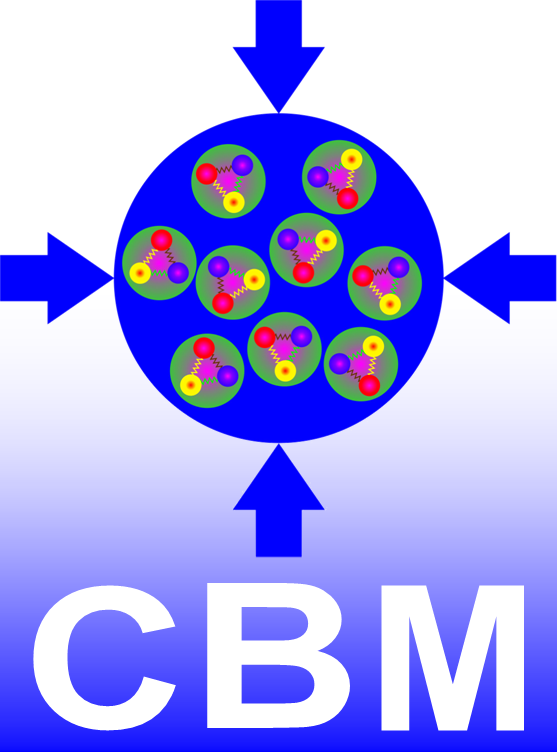
\includegraphics[width=0.66\textwidth]{gsi.png}
\end{center}
\newpage
\renewcommand{\abstractname}{Introduction}
\renewcommand{\thesection}{\Roman{section}.}
\renewcommand{\thesubsection}{\thesection.\arabic{subsection}.}
\renewcommand{\thesubsubsection}{\thesubsection.\arabic{subsubsection}.}
\begin{abstract}
	\par I have spent one month in summer at the GSI facility, Darmstadt to study the CBM simulation which will be part of FAIR$^{[1]}$. During this month I have become experienced with software such as ROOT$^{[2]}$, cbmROOT$^{[3]}$, etc.
	\vspace{5mm}
	\par I have learned much about detector technologies and natural phenomena during my stay and I was happy to be part of this huge project and see how scientist work on a daily basis and get the taste of that.
\end{abstract}
\tableofcontents
\newpage
\section{Fundamentals}
\par The CBM experiment is about to explore the highly compressed nuclear matter. The project is in construction phase and will be ready around 2020. Its unique feature is going to be the high luminosity of interactions and the online data processing.
\vspace{5mm}
\par The experiment intends to map the phase diagram of strongly interacting matter and to find out more about the early stages of the universe, neutron stars an probes QCD$^{[4]}$, the theory behind all of this.
\vspace{5mm}
\par It promises to explore the yet unknown areas of the phase diagram by heavy ion collisions. The research program is focused on vector mesons, $J/\Psi$, and multistrange hyperons.
\end{document}